\documentclass{article}[8pt]

\usepackage{minted}
\usepackage{fontspec}
\usepackage{tikz}
\usepackage{parskip}
\usepackage[margin=1cm]{geometry}
\usepackage{hyperref}

\usetikzlibrary{arrows,automata}
\setmainfont{Roboto}
\setmonofont{Hack}
\setminted{tabsize=4, style=friendly, fontsize=\footnotesize}
\pagenumbering{gobble}

\newcommand{\code}[1]{\textbf{\textit{#1}}}
\newcommand{\closed}{\code{Closed}}
\newcommand{\open}{\code{Open}}
\newcommand{\locked}{\code{Locked}}
\newcommand{\close}{\code{Close}}
\newcommand{\lock}{\code{Lock}}
\newcommand{\unlock}{\code{Unlock}}

\begin{document}

\section*{Introduction}
In my previous article (\href{https://sii.pl/blog/implementing-a-state-machine-in-c17/}{link}) we've talked about implementing a simple state machine based on a \code{std::variant} and other newer additions to the C++ standard.
Even though the implementation had it's merits it was far from being complete. In this article we improve upon that design to make it more useful and easy to use. If you haven't read the first part, I highly recommend that you do before diving into this article, as it heavily relies on code examples present there.

\section*{A problem to solve}

Let's start with defining a problem that'll serve as a testbed for new ideas. Previously a state machine representing basic door was used as an example. Sadly a door that anyone can open is not very useful, so let's change that. Let's introduce a new state \locked{} so that only somoeone who knows the key could open the door. A sequence diagram for such state machine could look like this:

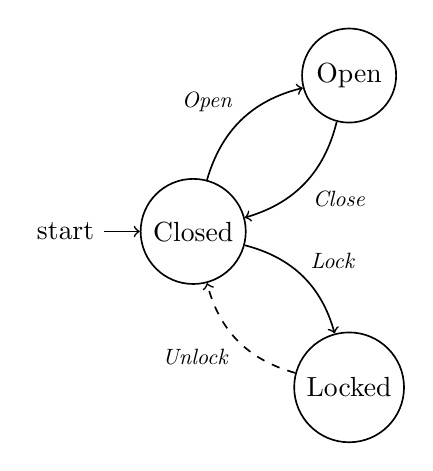
\begin{tikzpicture}[->, semithick, auto, node distance=2.8cm]
  \node[state, initial] (Closed) {Closed};
  \node[state]         (Open) [above right of=Closed] {Open};
  \node[state]         (Locked) [below right of=Closed] {Locked};

  \path (Closed) edge [bend left] node [scale=0.8] {\textit{Lock}}   (Locked)
			     edge [bend left] node [scale=0.8] {\textit{Open}}   (Open)
	    (Open)   edge [bend left] node [scale=0.8] {\textit{Close}}  (Closed)
	    (Locked) edge [dashed, bend left] node [scale=0.8] {\textit{Unlock}} (Closed);
\end{tikzpicture}

Besides an additional state, we've introduced two new events \lock{} and \unlock{}. Now, once the door is locked, the only way to open it is to unlock it first. With all that in mind, we can try to implement such state.

\bigskip
\begin{minted}{c++}
struct LockedState
{
	Nothing handle(const OpenEvent&) const { return {}; }
	Nothing handle(const CloseEvent&) const { return {}; }
	Nothing handle(const LockEvent&) const { return {}; }
	TransitionTo<UnlockedState> handle(const UnlockEvent&) const { return {}; };
};
\end{minted}
\bigskip

Now, that's a lot of boilerplate code! The state reacts only on \unlock{} event but we had to provide actions for all 4 events. To make it even worse, we need to implement handlers for those two newly added events in \closed{} and \open{} states. To fix this, let's provide a mechanism to collapse all similiar event handlers.

\bigskip
\inputminted[firstline=3]{c++}{../fsm/actions/ByDefault.h}
\bigskip

We can use this struct as a base for some of our states introducing some common behaviour. Why is the action type parametrized you might ask? That's because sometimes there's a better action to invoke other than \code{Nothing}, like for example
\\\code{TransitionTo<ErrorState>}. Let's see how this improves things when applied to \closed{} state.

\bigskip
\begin{minted}{c++}
struct ClosedState : ByDefault<Nothing>
{
	using ByDefault:handle;

	TransitionTo<LockedState> handle(const LockEvent&) const { return {}; }
	TransitionTo<OpenState> handle(const OpenEvent&) const { return {}; };
};
\end{minted}
\bigskip

Better! But still not perfect :) . First of all, as we have \code{handle} method overloaded in \code{ClosedState}, we need to pull \code{handle} from \code{ByDefault} base class with a \code{using} declaration.
Additionally, handlers for \code{LockEvent} and \code{OpenEvent} don't do anything except returning a default constructed action object. This behaviour could be shared in a helper base structure.

\bigskip
\inputminted[firstline=3]{c++}{../fsm/actions/On.h}
\bigskip
\begin{minted}{c++}
struct ClosedState : ByDefault<Nothing>,
					 On<LockEvent, TransitionTo<LockedState>>,
					 On<OpenEvent, TransitionTo<OpenState>>
{
	using ByDefault::handle;
	using On<LockEvent, TransitionTo<LockedState>>::handle;
	using On<OpenEvent, TransitionTo<OpenState>>::handle;
};
\end{minted}
\bigskip

Not much of an improvement since we still need to pull in handlers from all base classes. Fortunately there's a way to circumvent it. C++17 allows expanding parameter packs inside \code{using} declarations. We can use it to pull all overloads into a single base class.

\bigskip
\inputminted[firstline=3]{c++}{../fsm/actions/Will.h}
\bigskip

Now we can get rid of all those \code{using} declarations.

\bigskip
\begin{minted}{c++}
struct ClosedState : public Will<ByDefault<Nothing>,
								 On<LockEvent, TransitionTo<LockedState>>,
								 On<CloseEvent, TransitionTo<ClosedState>>>
{
};
\end{minted}
\bigskip

Now, that's much better :) . But our work is still far from complete. Even though we introduced a new \locked{} state, we still don't do any kind of verification. First of all we need to store some value, let's call it 'key', inside the state, which will be later used for access control. The issue here is that the states are currently default initialized by the state machine. We need to add a way to construct the states outside the state machine and pass them to the state machine constructor.

\bigskip
\begin{minted}{c++}
StateMachine() = default;

StateMachine(States... states)
	: states(std::move(states)...)
{
}
\end{minted}
\bigskip

In essence, when we're in a \locked{} state we should only accept \unlock{} events that have a matching 'key'. This poses a problem, since actions are returned from state \code{handle} methods and can have only one return type. We need to model somehow a situation where the result of an event can be an alternative of many possibilities. We can utilize \code{std::variant} for this task.

\bigskip
\begin{minted}{c++}
template <typename... Actions>
class OneOf
{
public:
	template <typename T>
	OneOf(T&& arg)
		: options(std::forward<T>(arg))
	{
	}

	template <typename Machine>
	void execute(Machine& machine)
	{
		std::visit([&machine](auto& action){ action.execute(machine); }, options);
	}

private:
	std::variant<Actions...> options;
};
\end{minted}
\bigskip

And since, most of the time, we want to either do one thing or do nothing at all, as a convenience, another helper type can be introduced.

\bigskip
\inputminted[firstline=5]{c++}{../fsm/actions/Maybe.h}
\bigskip

Now, with that in place, we can update both the \unlock{} event and \locked{} state

\bigskip
\begin{minted}{c++}
struct UnlockEvent
{
	uint32_t key;
};

class LockedState : public ByDefault<Nothing>
{
public:
	using ByDefault::handle;

	LockedState(uint32_t key)
		: key(key)
	{
	}

	Maybe<TransitionTo<ClosedState>> handle(const UnlockEvent& e) const
    {
        if (e.key == key) {
            return TransitionTo<ClosedState>{};
        }
        return Nothing{};
    }

private:
    uint32_t key;
};
\end{minted}
\bigskip

Great! That's exactly what we wanted! We've defined a state machine that reasembles a door that can by unlocked only when the passed event matches.

\section*{Taking things further}

What if we wanted to model some kind of programmable door. Like a safe in some hotels, were you can define your own pin code, but you can do that only when the safe is unlocked. We can add a 'newKey' field to \lock{} event. That's not a big problem. The biggest hurdle is how to inform \locked{} state about that new value? We could, for example, define a new action type that would update a given state. Even though that would solve our problem, it's not the best solution, since it requires \closed{} state to know the internals of a completely different state - \locked{}. The true problem that we need to solve lies even deeper. Instead of trying to pass this information from one state to the other, we should focus on giving the state information when it was entered and under what circumstances. For example, we could use this information to open a socket or maintain a database connection for as long as we're in that state and tear down everything once we leave.

To start, we need to provide a bit more information to the actions. In order to call apropriate methods \code{TransitionTo} action would need to know what's the current state and what event triggered the action. Apart from that, we want to grab a reference to the newly selected state when we make a transition. Let's update our state machine's implementation to provide that extra information.

\bigskip
\begin{minted}{c++}
template <typename Event>
void handle(const Event& event)
{
	auto passEventToState = [this, &event] (auto statePtr) {
		auto action = statePtr->handle(event);
		action.execute(*this, *statePtr, event);
	};
	std::visit(passEventToState, currentState);
}

template <typename State>
State& transitionTo()
{
	auto& state = std::get<State>(states);
	currentState = &state;
	return state;
}
\end{minted}
\bigskip

Now let's update the \code{TransitionTo} action. We want to call \code{onLeave} method on previous state and \code{onEnter} on the destination state, but how do we know that these methods are present? We could enforce it, just like it's done with \code{handle} methods, but that would lead to a lot of unnecessary code. We can use SFINAE (\href{https://en.cppreference.com/w/cpp/language/sfinae}{link}) to detect if such method exists. If it does, we'll call it, if not, we'll simply ignore it. You may ask why we didn't use that trick with \code{handle} methods and implemented a bunch of helpers just to provide some default behaviour? That's because the situation is a little bit different. Formally speaking, a transition function should be defined for each state and each event. Furthermore there are situations when we want to trigger a compilation error when we add a new event and one of the existing states doesn't know how to handle it, instead of blindly ignoring it. With that in mind, let's update the \code{TransitionTo} action.

\bigskip
\inputminted[firstline=3]{c++}{../fsm/actions/TransitionTo.h}
\bigskip

Thanks to SFINAE, we can detect if a \code{onEnter} or \code{onLeave} method was defined and act accordingly. The last thing to do is to implement an \code{onEnter} method for \locked{} state

\bigskip
\begin{minted}{c++}
void onEnter(const LockEvent& e)
{
	key = e.newKey;
}
\end{minted}
\bigskip

\section*{Wrapping things up}
In this article we explored how previous state machine implementation could be enhanced to support optional transitions and how to make it easier to use. States can now define custom \code{onEnter} and \code{onLeave} methods that will be called when the state is entered or left. If you want to play with that code, you can grab it \href{https://github.com/AdamsPL/state-machine}{here}.

In next part of the article we'll play with adding support for tracing and debugging information and we'll try to generate a nice transition table from the StateMachine type so stay tuned! :)
\end{document}
